\chapter{Background And Related Works}\label{ch:background}
Our investigation of existing works will consider three domains: The existing tools within Cogent,
termination and recursive types and linear and uniqueness types.

\section{Cogent Currently}
\todo{Type up}

\section{Termination And Recursive Types}

Proving total correctness about the programs we write is a very desirable result,
as computation performed by a program is useless if the program never returns the
result of the computation we desire.
In a systems context, this is especially desirable as an infinitely looping component of a
system could cause it to hang to hang, ruining the experience for end users of the system.

Our focus for reasoning about termination falls on considering the use of Isabelle to verify our 
embedding as well as facilitating the ease of this process at the type level within Cogent. 

\subsection{Proving Termination in Isabelle}


The official Isabelle tutorial\citep{IsabelleTutorial} describes 3 methods of creating functions using the keywords 
\textbf{primrec}, \textbf{fun} and \textbf{function}. The first, \textbf{primrec}, allows one to create a 
\textit{primitive recursive} function - one that returns a constant or removes a data type constructor from one
of the arguments to the function in its body, `decreasing' in size every time. These functions are \textit{total}
and always terminate, removing the need of a termination proof (which is required for all functions within Isabelle,
unless they are defined to be partial, however this is undesirable).
Primitive recursive functions however are limited in their expressiveness and are a subset of all computable
functions, so we cannot rely on them for the general case.

In his tutorial\citep{KraussIsabelle}, Alexander Krauss discusses the details of the latter two of the 3 methods
of creating functions in Isabelle. The \textbf{fun} keyword instructs Isabelle to try and solve all necessary
termination proof obligations, rejecting the definition if it fails (either because the definition does not 
terminate or because Isabelle cannot figure out how to prove it does). In contrast to this, \textbf{function}
requires that the termination proofs be solved manually by whoever is writing the proof.

\amos{Worth comparing the `gas' or `clock' approach as well, as used by CakeML (see CakeML: A Verified Implementation of ML, POPL 2014).
There, the embedding of the program has an extra parameter which is a natural number describing how much time the program has to compute a result.
At each recursive step, the clock is decremented, and if it reaches zero the program runs out of time and throws an exception.
This lets you embed arbitrary programs as primitive recursion on a nat.
You have to prove termination separately, but you can reason about the program assuming termination (assume that there exists a large enough clock that the program will return a valid value).}

\todo{Relate to proposal}

\subsection{Strictly Positive Types}

Adding recursive types to a type system allows for expressions that are potentially infinitely recursive,
as discussed by Wadler~\cite{RecursiveTypesForFree}, who explains the potential for recursive expressions
to cause non-termination through polymorphic lambda calculus. In his paper, he discusses how this
quality can be qualified with positive and negative data types.

Suppose a data type in its general form $T$ and its data constructors $C_{1..n}$, each with a number of arguments 
$\tau_{i1}..\tau_{ik}$:

\begin{center}
    \begin{tabular}{l}
        $T = C_1\; \tau_{11} \; \tau_{12} \; \dots$ \\
        $\hspace{1.5em} \vert\; C_2\; \tau_{21} \; \tau_{22} \; \dots$ \\
        $\hspace{1.5em} \vert\; \dots$ \\
    \end{tabular} 
\end{center}

\theoremstyle{definition}
\begin{definition}
    A data type $T$ is said to be in a \textit{negative position} if $T$ appears nested as an argument
    to a function an odd amount of times inside any $\tau_{ij}$, and said to be in a \textit{positive position}
    if $T$ appears nested as an argument to a function an even amount of times inside $\tau_{ij}$.
\end{definition}

\theoremstyle{definition}
\begin{definition}
    A data type $T$ is a \textit{negative} data type if it appears in a negative position 
    in one of its constructors.
\end{definition}

\theoremstyle{definition}
\begin{definition}
    A data type $T$ is a \textit{positive} data type if only appears nested in a positive position
    in all of its constructors.
\end{definition}

In simpler terms, if $T$ appears to the left of a function arrow an odd amount of times, it is negative and if
to the left an even amount of times then it is positive.

For example:

\begin{center}
    \begin{tabular}{l}
        $E = C\; (\underline{E} \rightarrow E)$ \\
        $K = D\; (\underline{(\underline{K} \rightarrow_1 Int)} \rightarrow_2 K)$
    \end{tabular} 
\end{center}

Here, the data type $E$ is negative as it appears in a negative position (denoted here by an underline)
to a function in the first argument of $C$.
$K$ however is positive as it appears only ever in a positive position as it is nested as an argument
in function 1 ($\rightarrow_1$) and again in function 2 ($\rightarrow_2$) for a total of two times.

Allowing for negative types in our system allow for data structures that are infinitely recursive,
which if iterated over would potentially cause non-termination. Consider
the following example in \textit{Haskell}:

\lstinputlisting[language=haskell]{content/NegativeType.hs}

By our definition, we can see that our type \textit{Bad} is a \textit{negative} type and using it we were able
to construct the infinitely recursive expression, \textbf{g (A g)}.
This is not an issue in Haskell due to its lazy evaluation,
however as Cogent is not lazily evaluated these expressions would be undesirable in
our language as iterating over them potentially results in non-termination, and in this
situation hang when \textit{infiniteExpression} is constructed.
Although this example was constructed maliciously, situations may arise where
programmers may accidentally construct such an expression, so we must seek a way to
eliminate them from our language.

Many theorem provers and dependently typed languages make use of \textit{strictly positive} types, which
prohibit the construction of infinitely recursive data structures that under a dependant type system
both negative and simple positive types allow.
\textit{Agda}\citep{AgdaStrictlyPositive}, \textit{Coq}\citep{CoqStrictlyPositive} and even
Isabelle\citep{IsabelleStrictlyPositive} do exactly this, as allowing for negative or simple positive
types introduce logical inconsistencies which can be used to prove false statements.

The definition of strictly positive is discussed by Coquand and Paulin~\cite{CoquandTypes}, and is as follows:

\theoremstyle{definition}
\begin{definition}
    \label{def:sp}
    Given a data type $T$ and its constructors $C_{1..n}$, for every argument $\tau_{ij}$
    of any data constructor $C_i$ wher $\tau_{ij}$ is a function, $T$ is said to be \textit{strictly positive} if 
    $T$ does not occur as an argument to any $\tau_{ij}$:

    \begin{center}
        $\forall\; \tau_{ij}.\;
        (\tau_{ij} = \phi_{1} \rightarrow \dots \rightarrow \phi_{k})
        \implies T \notin \phi_{1..k-1}$
    \end{center}
\end{definition}

Strictly positive types can also be defined as types where $T$ appears in a negative or positive 
position exactly zero times (i.e. it does not appear to the left of any arrow).

In their paper, Conquand and Paulin further discuss the ability to produce an \textit{eliminator} or a
\textit{fold} from any strictly positive type --- which corresponds to an induction principle on the type.

Consider a type for natural numbers with two constructors for zero and successor:

\begin{center}
    \begin{tabular}{l}
        $Nat = \textsc{Z}\; \vert\; \textsc{S}\; Nat$ \\
    \end{tabular} 
\end{center}

We can see $Nat$ is a strictly positive type and the induction principle it produces
for any predicate over natural numbers, $P$, is:

\[
    \infer{
        \forall(N : Nat).\;\; P(N)
    }{
        P(Z) \quad & \forall (X : Nat).\; P(X) \implies P(S\; X)
    }
\]

That is, to prove any predicate $P$ inductively over nats ($\forall(N : Nat).\; P(N)$)
we provie it for the base (zero) case $P(Z)$ and then assuming the predicate holds
for a natural number $X$, we prove it for its successor case $S\; X$: $P(X) \implies P(S\; X)$.

The interactive theorem prover Isabelle does exactly this for any type created in Isabelle. We can 
get the same induction principle over natural numbers by redefining our $Nat$ type in Isabelle, as in 
figure \ref{fig:IsabelleNatInduct}.

\begin{center}
    \begin{figure}
        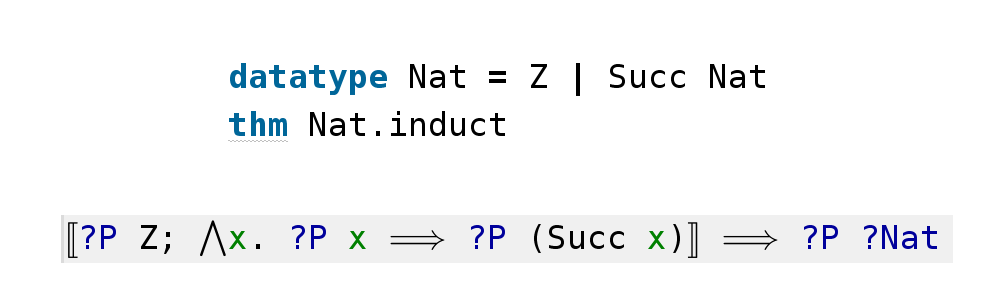
\includegraphics[width=\linewidth]{content/isabelleNatInduct.png}
        \caption{A type for natural numbers defined in Isabelle, and the generated 
        induction principle associated with the type.}
        \label{fig:IsabelleNatInduct}
    \end{figure}
\end{center}

\FloatBarrier

Considering our Cogent embedding will be within Isabelle, we may potentially be able to 
get Isabelle to generate an induction principle over our Cogent types, allowing for much 
simpler reasoning about our Isabelle embedding.

\section{Linear \& Uniqueness Types}
\todo{Type up}